\documentclass[11pt]{article}
\input{/Users/markwang/.preamble}
\begin{document}


% arg1=pdfurl arg2=pagenum arg3=sectiontitle
\newcommand{\linksection}[3][../../bishop_pattern_recognition_and_machine_learning.pdf]{
    \subsection*{\href[page=#2]{#1}{#3}}
}

\newcommand{\linkinline}[3][../../bishop_pattern_recognition_and_machine_learning.pdf]{
    \noindent\href[page=#2]{#1}{#3}
}

\renewcommand{\norm}[1]{\left\lVert#1\right\rVert}
\renewcommand{\E}[2][]{\mathbb{E}_{#1}\left\{#2\right\}}
\newcommand{\var}[2][]{var_{#1}\left\{#2\right\}}
\newcommand{\cov}[1]{cov\{#1\}} 
\newcommand{\normal}[1]{\mathcal{N}\left(#1\right)}
\newcommand{\exponents}[1]{exp\left\{#1\right\}}

\newcommand{\bmu}{\boldsymbol{\mu}}
\newcommand{\bpi}{\boldsymbol{\pi}}
\newcommand{\bTheta}{\boldsymbol{\Theta}}
\newcommand{\bSigma}{\boldsymbol{\Sigma}}
\newcommand{\bphi}{\boldsymbol{\phi}}

\newcommand{\calL}{\mathcal{L}}
\newcommand{\calE}{\mathcal{E}}
\newcommand{\calR}{\mathcal{R}}
\newcommand{\calC}{\mathcal{C}}
\newcommand{\calD}{\mathcal{D}}
\newcommand{\bx}{\matr{x}}
\newcommand{\bt}{\matr{t}}
\newcommand{\bw}{\matr{w}}
\newcommand{\bX}{\matr{X}}
\newcommand{\bZ}{\matr{Z}}
\newcommand{\bz}{\matr{z}}
\newcommand{\bu}{\matr{u}}



\newcommand{\lebpar}[2]{\frac{\partial #1}{\partial #2}}
\newcommand{\qqqquad}{\quad \quad \quad \quad}

% function for conditional independence
% https://tex.stackexchange.com/questions/218631/symbol-for-not-conditionally-independent
\newcommand{\bigCI}{\mathrel{\text{\scalebox{1.07}{$\perp\mkern-10mu\perp$}}}}
\newcommand{\nbigCI}{\centernot{\bigCI}}

\newcommand{\condi}[3]{#1 \bigCI #2 \,|\, #3}
\newcommand{\notcondi}[3]{#1 \nbigCI #2 \,|\, #3}





\linksection{574}{13 Sequential Data}


\begin{enumerate}   
    \item \textbf{Stationary sequential distribution}
    \item \textbf{Markov Model} assume future prediction depends on the most recent observations
    \item \textbf{State Space Model} 
\end{enumerate}


\begin{defn*}
    \textbf{Markov Model} models observations that are not i.i.d. If each of conditional distribution is independent of all previous observations except the most recent, then we obtain first-order Markov chain, 
    \begin{center}
        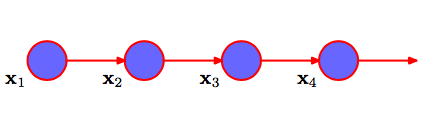
\includegraphics[width=6cm]{first_order_markov_chain.png}
    \end{center} 
    \[
        p(\bx_1, \cdots, \bx_N) 
        \overset{product\,rule}{=} \prod_{n=1}^N p(\bx_n | \bx_1, \cdots, \bx_{n-1})
        \overset{markov}{=} p(\bx_1) \prod_{n=2}^N p(\bx_n | \bx_{n-1})
    \]
    the distribution of prediction depends only on value of immediate preceding observation 
    \[
        p(\bx_n | \bx_1 ,\cdots, \bx_{n-1}) = p(\bx_n | \bx_{n-1})
    \]
    where $p(\bx_n | \bx_{n-1})$ is fixed and hence the model is \textbf{stationary}. We can extend to $M^{th}$ order Markov chain in which the conditional distribution for a particular variable depends on the previous $M$ variables. However we have exponentially more parameters to maintain. So instead we introduce latent variables to the Markov chain, with each observation conditioned on the state of the corresponding latent variable. This gives rise to \textbf{hidden markov model} if latent variable is discrete and \textbf{linear dynamic systems} if both latent and observed variables are Gaussian.
    \begin{center}
        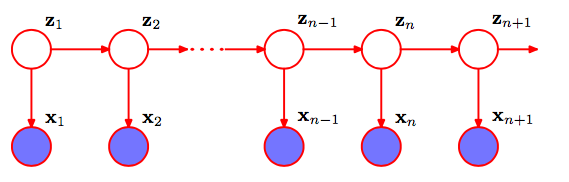
\includegraphics[width=7cm]{hmm.png}
    \end{center}
    \[
        p(\bx_1, \cdots, \bx_N, \bz_1, \cdots, \bz_N)
        = p(\bz_1) \prod_{n=2}^N p(\bz_n | \bz_{n-1}) \prod_{n=1}^N p(\bx_n | \bz_n)
    \]
    and we note $\condi{\bz_{n+1}}{\bz_{n-1}}{\bz_n}$. Also, there is always a nonblocking path connecting any observation. So any prediction for $\bx_{n+1}$ does not exhibit conditional independence property, so depends on all previous observations $\bx_1, \cdots, \bx_n$
\end{defn*}

\newpage

\begin{defn*}
    \textbf{Hidden Markov Model} 
    \begin{enumerate}
        \item \textbf{Model Formulation} Like mixture model where choice of mixture component for each observation not selected independently but depends on choice of component for previous observation. Latent variables are discrete multinomial varaible $\bz_n$ describing which component of mixture is responsible for generating the corresponding observations. We assume a constant \textbf{transition probability} $\matr{A}$ cross all hidden states
        \[
            A_{jk} = p(z_{nk}=1 | z_{n-1,j} = 1)
            \qquad 0\leq A_{jk}\leq 1 
            \quad \sum_k A_{jk} = 1
        \]
        i.e. transition probability from picking $j$-th component to picking $k$-th component. We define $\bpi$ be \textbf{initial probability} for $\bz_1$ since it does not have parent node, in other words $\pi_k = p(z_{1k}=1)$. Therefore we can define probability distribution for edges connecting hidden states $p(\bz_n | \bz_{n-1}, \matr{A})$ and $p(\bz_1 | \bpi)$
        \[
            p(\bz_n | \bz_{n-1}, \matr{A}) = \prod_{k=1}^K \prod_{j=1}^K (A_{jk})^{z_{n-1, j} z_{nk}}
            \qquad 
            p(\bz_1 | \bpi) = \prod_{k=1}^K \pi_k^{z_{1k}}
        \]
        We define \textbf{emission probabilities} as $p(\bx_n | \bz_n , \bphi)$ be responsible for converting state paths into a sequence of observable varaibles. $\bphi$ is a set of parameters governing the distribution that is constant cross all emission probabilities under a homogeneous model. The emission probability consists of $K$ possible different distributions corresponding to $K$ possible states of $\bz_n$ 
        \[
            p(\bx_n | \bz_n , \bphi)=  \prod_{k=1}^K p(\bx_n | \bphi_k)^{z_{nk}}    
        \]
        Therefore the \textbf{joint distribution} of both observed and latent varaibles is given by 
        \[
            p(\bX, \bZ | \bTheta) = p(\bz_1 | \bpi) \prod_{n=2}^N p(\bz_n | \bz_{n-1}, \matr{A}) \prod_{m=1}^N p(\bx_m | \bz_m, \bphi)    
        \]
        given $\bTheta = \{ \bpi, \matr{A}, \bphi \}$. 
        \item \textbf{A Generative View} we can treat HMM as follows 
        \begin{enumerate}
            \item pick initial latent variable $\bz_1$ given $\bpi$, then sample $\bx_1$
            \item choose next latent variable using $\matr{A}$, then sample from the emission probabilities
        \end{enumerate}
        \item \textbf{MLE for HMM} Given dataset $\bX = \{\bx_1, \cdots, \bx_N\}$ want to determine parameter $\bTheta$ with maximum likelihood. Want to maximize the likelihood
        \[
            p(\bX | \bTheta) = \sum_{\bZ} p(\bX, \bZ | \bTheta)    
        \]
        which does not factor over $n$ easily. We first are concerned with evaluating computing $p(\bX | \bTheta)$ efficiently since we would have to consider $K^N$ different possible $Z$s, hence not feasible. We solve this by rearranging the summation such that the cost scales linearly instead of exponentially 
        \begin{align*}
            p(\bX | \bTheta)
            &= \sum_{\bZ} p(\bX, \bZ | \bTheta) \\ 
            &= \sum_{\bz_1, \cdots, \bz_n} p(\bz_1, \bx_1) \prod_{n=2}^N p(\bz_n | \bz_{n-1}) p(\bx_n | \bz_n)  \\ 
            &= \sum_{\bz_1} p(\bz_1) p(\bx_1 | \bz_1) \sum_{\bz_2} p(\bz_2 |\bz_1) p(\bx_2 | \bz_2) \cdots \sum_{\bz_N} p(\bz_{N} | \bz_{n-1}) p(\bx_N | \bz_N)
        \end{align*}
        which usually have no closed form. So we use EM algorithm 
        \item \textbf{Forward-Backward algorithm} Used for computing the posterior of hidden states over observation 
        \[
            p(\bz_n | \bX) = \frac{p(\bX | \bz_n)p(\bz_n)}{p(\bX)} = \frac{\alpha(\bz_n)\beta(\bz_n)}{p(\bX)}
        \]
        where the algorithm evaluates $\alpha(\bz_n)$ in terms of $\alpha_{\bz_{n-1}}$ and in the backward pass evaluates $\beta(\bz_n)$ in terms of $\alpha_{\bz_{n+1}}$. The algorithm can be used to compute likelihood $p(\bX | \bTheta)$ !
        \item \textbf{Baum-Welch algorithm} is EM for HMM
        \item \textbf{Viterbi Decoding} determines the most probable paths from exponentially many possibilities
    \end{enumerate}
\end{defn*}


\end{document}
